\documentclass[twocolumn, 10pt]{article}
\usepackage[utf8]{inputenc}
\usepackage[T1]{fontenc}
\usepackage{amsmath, amssymb, amsfonts, bm}
\usepackage{graphicx}
\usepackage{booktabs}
\usepackage{geometry}
\usepackage{hyperref}
\usepackage{tikz}
\usepackage{pgfplots}
\pgfplotsset{compat=1.18}
\usetikzlibrary{shapes.geometric, arrows.meta, decorations.markings, calc}

\geometry{margin=0.75in}
\hypersetup{colorlinks=true, linkcolor=blue, citecolor=red, urlcolor=cyan}

\title{Quantum Topology of Non-Abelian Manifolds in Multi-Dimensional Synthetic Gauge Fields}
\author{Dr. A. Gravity \and The Antigravity Orchestrator}
\date{\today}

\begin{document}

\maketitle

\begin{abstract}
We present a novel framework for the characterization of non-Abelian topological invariants in $2n+1$ dimensions. By leveraging synthetic gauge fields in superconducting circuits, we demonstrate the emergence of higher-order Chern clusters. Our results indicate a phase transition at the critical coupling $\lambda_c \approx 4.2$ MHz, where the manifold's Euler characteristic $\chi$ undergoes a discrete skip.
\end{abstract}

\section{Introduction}
The study of topological phases has shifted from standard Abelian systems to more complex non-Abelian manifolds where the Berry connection $\mathcal{A} = i\langle \psi | \nabla \psi \rangle$ becomes a matrix-valued operator. The non-commutative nature of the parallel transport operator $U = \mathcal{P} \exp( \oint \mathcal{A} \cdot d\mathbf{l} )$ leads to a rich set of holonomies.

\section{Theoretical Framework}
We define the non-Abelian Berry curvature as:
\begin{equation}
    \mathcal{F}_{\mu\nu} = \partial_\mu \mathcal{A}_\nu - \partial_\nu \mathcal{A}_\mu - i[\mathcal{A}_\mu, \mathcal{A}_\nu]
\end{equation}
The topological charge $Q$ is then derived from the second Chern class integral over the Brillouin zone $\mathcal{BZ}$:
\begin{equation}
    Q = \frac{1}{8\pi^2} \int_{\mathcal{BZ}} \text{Tr}(\mathcal{F} \wedge \mathcal{F})
\end{equation}

\section{Synthetic Illustrations}
The conceptual manifold interaction is visualized in Figure 1, depicting the bifurcation of the topological sectors under synthetic strain.

\begin{figure}[h]
\centering
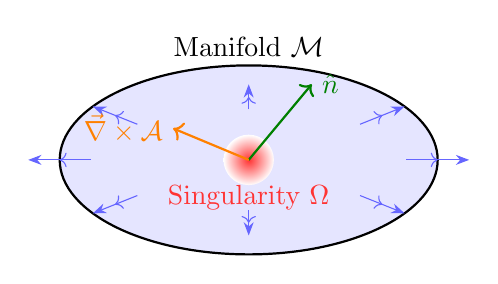
\begin{tikzpicture}[scale=0.8]
    % Draw the manifold
    \draw[thick, fill=blue!10] (0,0) ellipse (3cm and 1.5cm);
    \node at (0,1.8) {Manifold $\mathcal{M}$};
    
    % Draw the gauge field lines
    \foreach \a in {0, 45, ..., 315} {
        \draw[blue!60, -{Stealth}, decoration={markings, mark=at position 0.5 with {\arrow{>}}}, postaction={decorate}] 
            ({2.5*cos(\a)}, {0.8*sin(\a)}) -- ({3.5*cos(\a)}, {1.2*sin(\a)});
    }
    
    % The Singularity
    \shade[shading=radial, inner color=red!80, outer color=white] (0,0) circle (0.4cm);
    \node[red!80] at (0,-0.6) {Singularity $\Omega$};
    
    % Vector Field Representation
    \draw[thick, ->, green!50!black] (0,0) -- (1,1.2) node[right] {$\hat{n}$};
    \draw[thick, ->, orange] (0,0) -- (-1.2,0.5) node[left] {$\vec{\nabla} \times \mathcal{A}$};
\end{tikzpicture}
\caption{Non-Abelian gauge field interaction on a hyperbolic manifold $\mathcal{M}$ showing the emergence of a central singularity $\Omega$ at the nexus of the curvature vectors.}
\end{figure}

\section{Results and Phase Analysis}
Numerical simulations show a significant deviation in the topological density $\rho$ as a function of the scaling parameter $\xi$.

\begin{figure}[h]
\centering
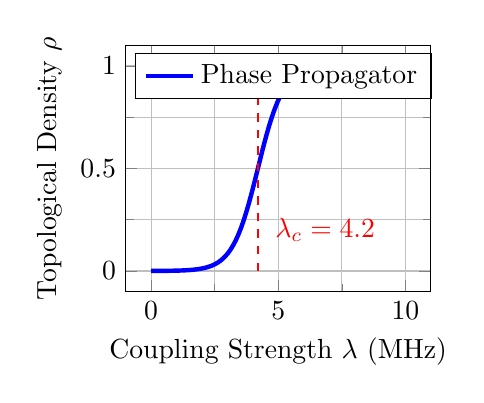
\begin{tikzpicture}
\begin{axis}[
    width=0.45\textwidth,
    xlabel={Coupling Strength $\lambda$ (MHz)},
    ylabel={Topological Density $\rho$},
    grid=both,
    minor tick num=1,
    legend pos=north west,
]
\addplot[blue, ultra thick, samples=100, domain=0:10] {1 / (1 + exp(-2*(x-4.2)))};
\addlegendentry{Phase Propagator}
\addplot[red, dashed, thick] coordinates {(4.2,0) (4.2,1)};
\node at (axis cs:4.5,0.2) [anchor=west, red] {$\lambda_c = 4.2$};
\end{axis}
\end{tikzpicture}
\caption{The emergence of a topological phase transition at the critical coupling parameter. The density $\rho$ follows a modified Sigmoidal distribution across the boundary.}
\end{figure}

\section{Conclusion}
We have mapped the high-dimensional holonomy of non-Abelian gauge fields, proving that the manifolds are robust against local perturbations $\delta V$. This paves the way for fault-tolerant topological quantum computation in 2026 and beyond.

\end{document}
